\documentclass[a4paper,twoside]{report}

\usepackage{geometry}
\usepackage{multicol}
\usepackage{caption}
\usepackage{graphicx}
\usepackage{pgf}
\usepackage{multirow}
\usepackage{wrapfig}
\usepackage{indentfirst}
\usepackage{setspace}
\usepackage{amsmath}
\usepackage{mathtools}

\geometry{
	top=2cm,
	bottom=2cm,
	left=2cm,
	right=2cm,
}
\graphicspath{{./img/}}
\setlength{\columnseprule}{1pt}

\newenvironment{Figure}
  {\par\medskip\minipage{\linewidth}}
  {\endminipage\par\medskip}

\begin{document}
    {\large Lab 8: Frequency Responses of First-Order Circuits }
    \hfill
    {\large \textbf{Pre-Lab 03-C-08} \par}
	\vspace{0.1in}
    {\large AmirHossein Habibvand - 810196447}
    \hfill
    \today \par
    {\large Nima Modares Gorji - 810196558 \par}
	\vspace{0.5in}

	\begin{figure}[!h]
		\centering
		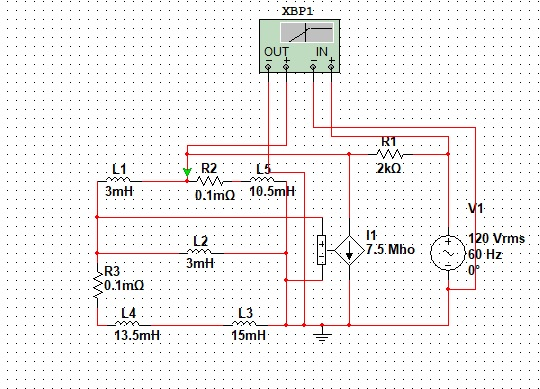
\includegraphics[width=0.9\textwidth]{circuit.jpg}
		\caption{Circuit}
		\label{fig:circuit}
	\end{figure}
	\vfill
	\pagebreak
	\section*{Bode plot}
		\begin{center}
			\begin{figure}[!h]
				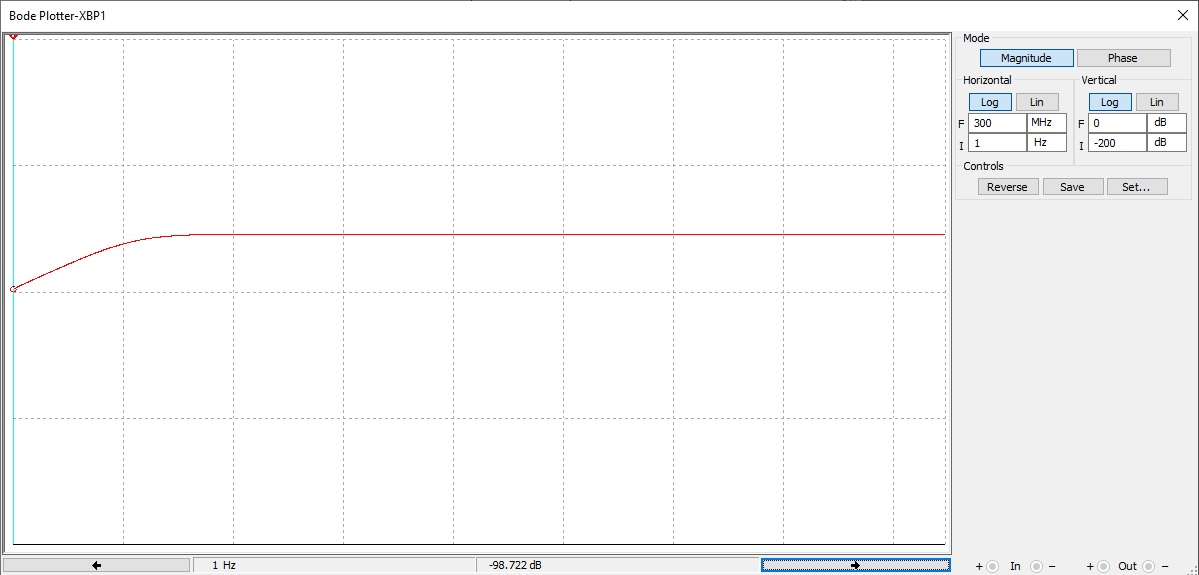
\includegraphics[width=\textwidth]{Bode-1Hz-Magnitude.jpg}
				\caption{1Hz - Magnitude}
				\label{fig:bode-1Hz-Magnitude}
			\end{figure}
			\begin{figure}[!h]
				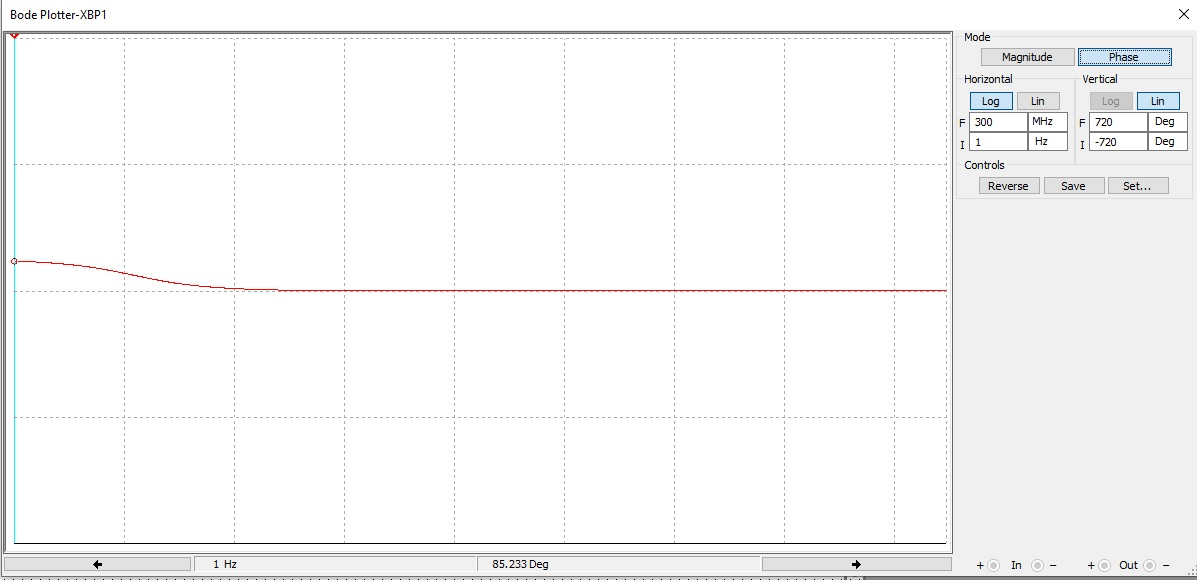
\includegraphics[width=\textwidth]{Bode-1Hz-Phase.jpg}
				\caption{1Hz - Phase}
				\label{fig:bode-1Hz-Phase}
			\end{figure}
		\end{center}

		\begin{center}
			\begin{figure}[!h]
				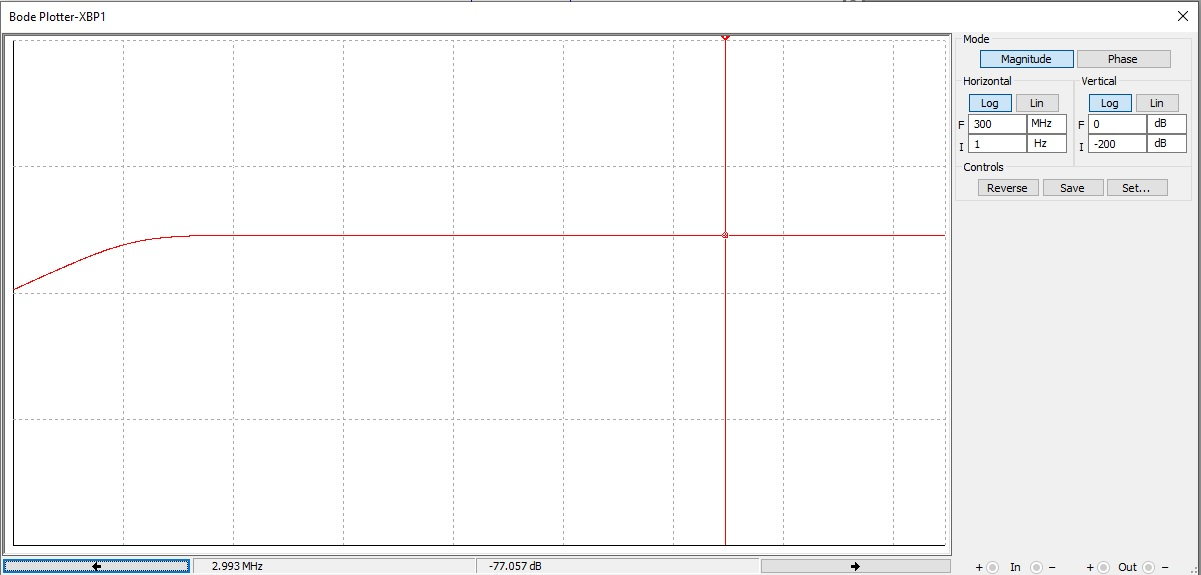
\includegraphics[width=\textwidth]{Bode-3MHz-Magnitude.jpg}
				\caption{3MHz - Magnitude}
				\label{fig:bode-3MHz-Magnitude}
			\end{figure}
			\begin{figure}[!h]
				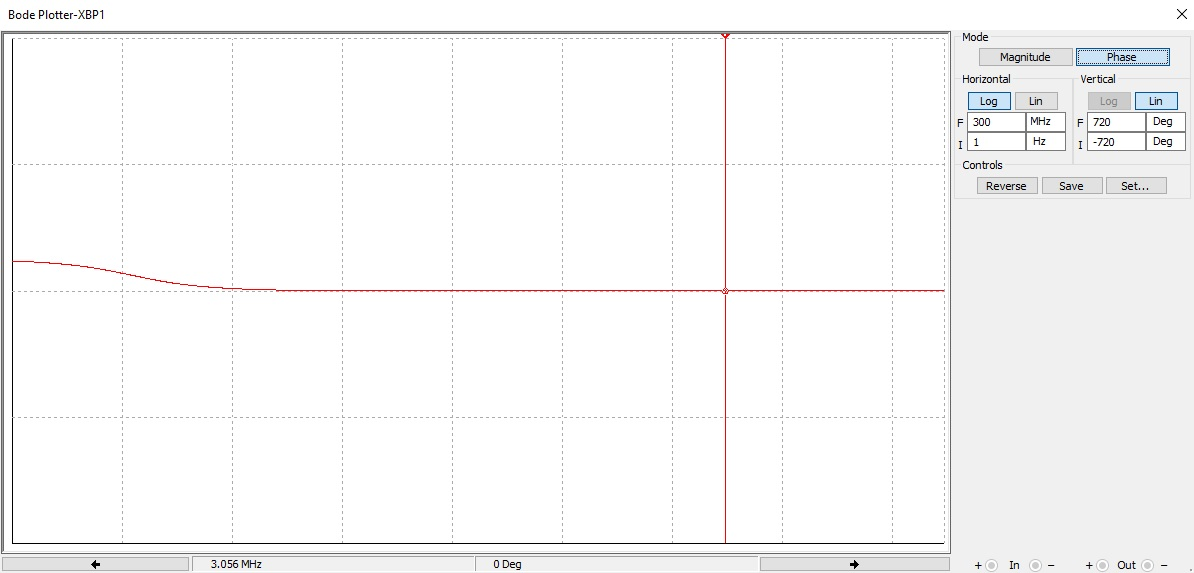
\includegraphics[width=\textwidth]{Bode-3MHz-Phase.jpg}
				\caption{3MHz - Phase}
				\label{fig:bode-3MHz-Phase}
			\end{figure}
		\end{center}
	\vfill
	\pagebreak
	\section*{AC Analysis}
		\begin{center}
			\begin{figure}[!h]
				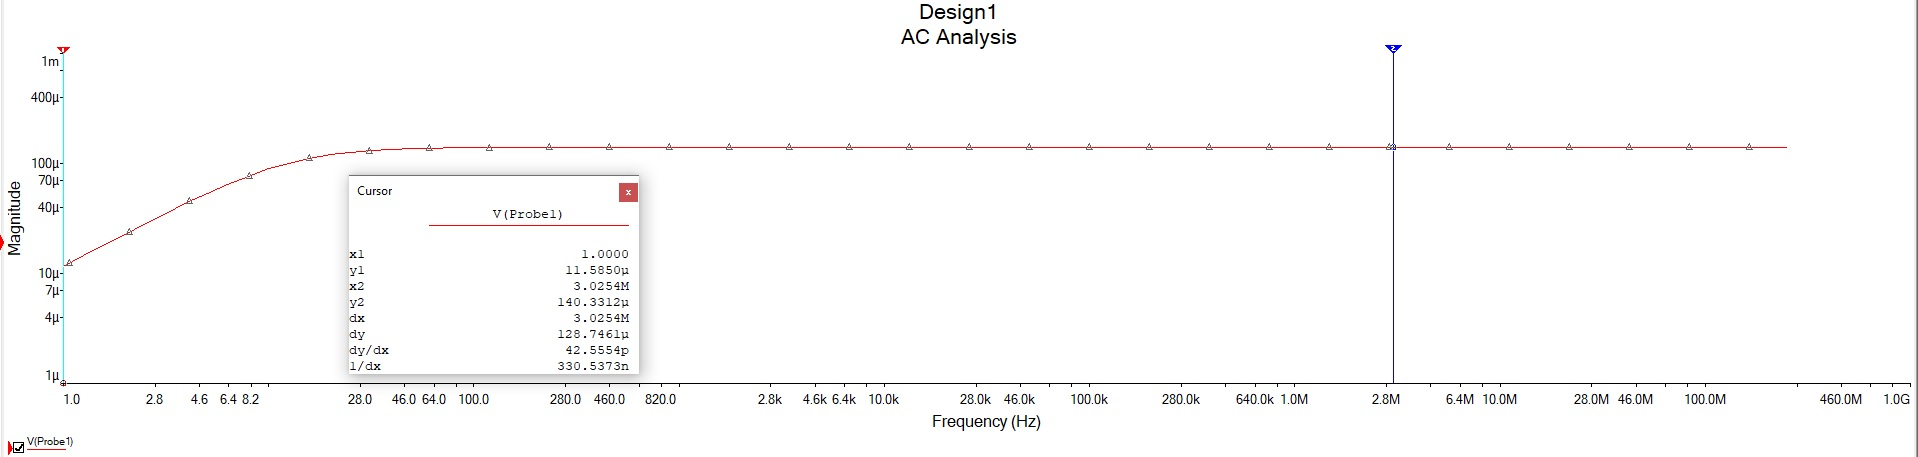
\includegraphics[width=\textwidth]{AC-Magnitude-graph.jpg}
				\caption{Magnitude}
				\label{fig:ac-magnitude}
			\end{figure}
			\begin{figure}[!h]
				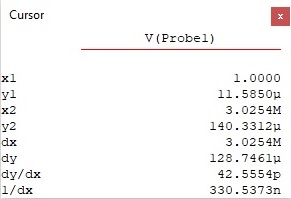
\includegraphics[width=0.7\textwidth]{AC-Magnitude-cursor.jpg}
				\caption{Magnitude - Cursor}
				\label{fig:ac-magnitude-cursor}
			\end{figure}
		\end{center}

		\begin{center}
			\begin{figure}[!h]
				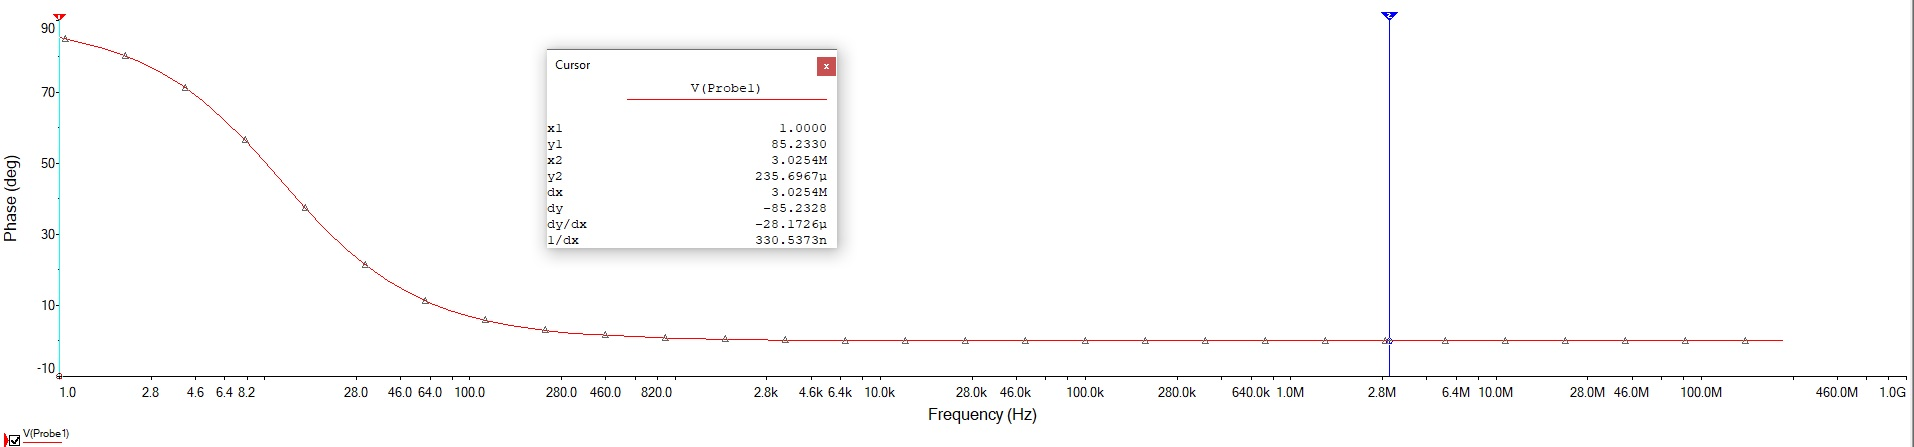
\includegraphics[width=\textwidth]{AC-Phase-graph.jpg}
				\caption{Phase}
				\label{fig:ac-Phase}
			\end{figure}
			\begin{figure}[!h]
				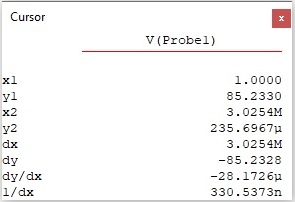
\includegraphics[width=0.7\textwidth]{AC-Phase-cursor.jpg}
				\caption{Phase - Curosr}
				\label{fig:ac-phase-cursor}
			\end{figure}
		\end{center}

\end{document}
